\documentclass[11pt,reqno,final]{amsart}

\pdfcompresslevel=0
\pdfobjcompresslevel=0

\usepackage[dvipsnames]{xcolor}% adds colors
\usepackage{amsmath, amsthm}% {amsfonts, amssymb}

% New Characters
\usepackage[latin1]{inputenc}%
\usepackage[T1]{fontenc}

\usepackage{MnSymbol}
\usepackage[normalem]{ulem}% underlining

\usepackage[theoremfont, largesc]{newpxtext} % different text,math font
\usepackage{newpxmath}

\makeatletter
\DeclareMathRadical{\sqrtsign}{symbols}{112}{largesymbols}{112}
% \let\sqrt=\undefined
% \DeclareRobustCommand\sqrt{\@ifnextchar[\@sqrt{\mathpalette\@x@sqrt}]}
% \def\@x@sqrt#1#2{%
%  \setbox\z@\hbox{$\m@th#1\sqrtsign{\mkern1mu #2}$}
%  \mkern3mu\box\z@}
\makeatother




% Page Typesetting
\usepackage[final]{microtype}
\usepackage{relsize}
\usepackage[margin=1in]{geometry}
\usepackage{framed}
\usepackage{tikz}

\usepackage{setspace}
\onehalfspacing

\usepackage{hyperref}
\hypersetup{
  final,
  pdftitle={Math 135 - The derivative, graphs, and first rules},
  pdfauthor={Bonventre}, 
  linktoc=page,
  pagebackref,
  colorlinks=true,
  citecolor=PineGreen,
  linkcolor=PineGreen,
  linkbordercolor=PineGreen,
}


% Internal References

\usepackage[inline,shortlabels]{enumitem}

% \numberwithin{equation}{section} 
\numberwithin{figure}{section}

\usepackage[nameinlink,capitalise,noabbrev]{cleveref}

\crefname{equation}{}{} % get \cref to behave as \eqref

% \theoremstyle{plain} % bold name, italic text
\newtheorem{theorem}[equation]{Theorem}%
\newtheorem*{theorem*}{Theorem}%
\newtheorem{lemma}[equation]{Lemma}%
\newtheorem{proposition}[equation]{Proposition}%
\newtheorem{corollary}[equation]{Corollary}%
\newtheorem{conjecture}[equation]{Conjecture}%
\newtheorem*{conjecture*}{Conjecture}%
\newtheorem{claim}[equation]{Claim}%
\newtheorem{question}{Question}

\theoremstyle{definition} % bold name, plain text
\newtheorem{definition}[equation]{Definition}%
\newtheorem*{definition*}{Definition}%
\newtheorem{example}[equation]{Example}%
\newtheorem*{example*}{Example}%
\newtheorem{remark}[equation]{Remark}%
\newtheorem{notation}[equation]{Notation}%
\newtheorem{convention}[equation]{Convention}%
\newtheorem{assumption}[equation]{Assumption}%
\newtheorem{exercise}[question]{Exercise}

% ---------- macros
\newcommand{\set}[1]{\left\{#1\right\}}%
\newcommand{\sets}[2]{\left\{ #1 \;|\; #2\right\}}%
\newcommand{\longto}{\longrightarrow}%
\newcommand{\into}{\hookrightarrow}%
\newcommand{\onto}{\twoheadrightarrow}%

\usepackage{harpoon}
\newcommand{\vect}[1]{\text{\overrightharp{\ensuremath{#1}}}}

\newcommand{\del}{\partial}%

\newcommand{\ki}{\chi}
\newcommand{\ksi}{\xi}
\newcommand{\Ksi}{\Xi}

\newcommand{\dlim}{\displaystyle\lim}

% %%%%%%%%%%%%%%%%%%%%%%%%%%%%%%%%%%%%%%%%%%%%%%%%%%%%%%%%%%%%%%%%%%%%%%%%%%%%%%%%%%%%%%%%%%%%%%%%%%%%

\begin{document}

\newgeometry{bottom=0in}


\begin{center}
        \textbf{\Large Math 135, Calculus 1, Fall 2020}\\[10pt]
        {\large 10-07: The Derivative, Graphs, and First Rules}
\end{center}

\thispagestyle{empty}


\renewcommand{\thesection}{\Alph{section}}

% \vspace{-1pt}

Recall the \textbf{derivative function} $f'(x)$ of a function $f(x)$ is defined to be
\begin{itemize}
\item the slope of the tangent line
\item the instantaneous velocity
\item $\dlim_{h \to 0}\dfrac{f(x+h) - f(x)}{h}$
\end{itemize}

\section{Graphs of $f'(x)$}

\begin{exercise}
        Consider the function $f(x) = x^2-x-2$.
        We will construct the graph of the derivative function one point at a time.
        \begin{enumerate}[(a)]
        \item Go to the website\  \url{http://www.shodor.org/interactivate/activities/Derivate/}.
        \item Enter the function $y = f(x)$ above. Use the tool to cacluate the slope of the tangent line at each of the points
                $x = -1,\ 0,\ 1,\ 2,$ and $2.5$.
                Enter these values in the table below:
                \begin{table}[hp]
                        \centering
                        \begin{tabular}{c||c|c|c|c|c}
                          $x$ & \ $-1$\ &\  0\ &\ 1\ &\ 2\ &\ 2.5\ \\ \hline
                          slope of $g$ at $x$ &&&&
                        \end{tabular}
                \end{table}
        \item Now plot these points and connect them smoothly to estiamte a graph of $f'(x)$.
                \begin{center}
                        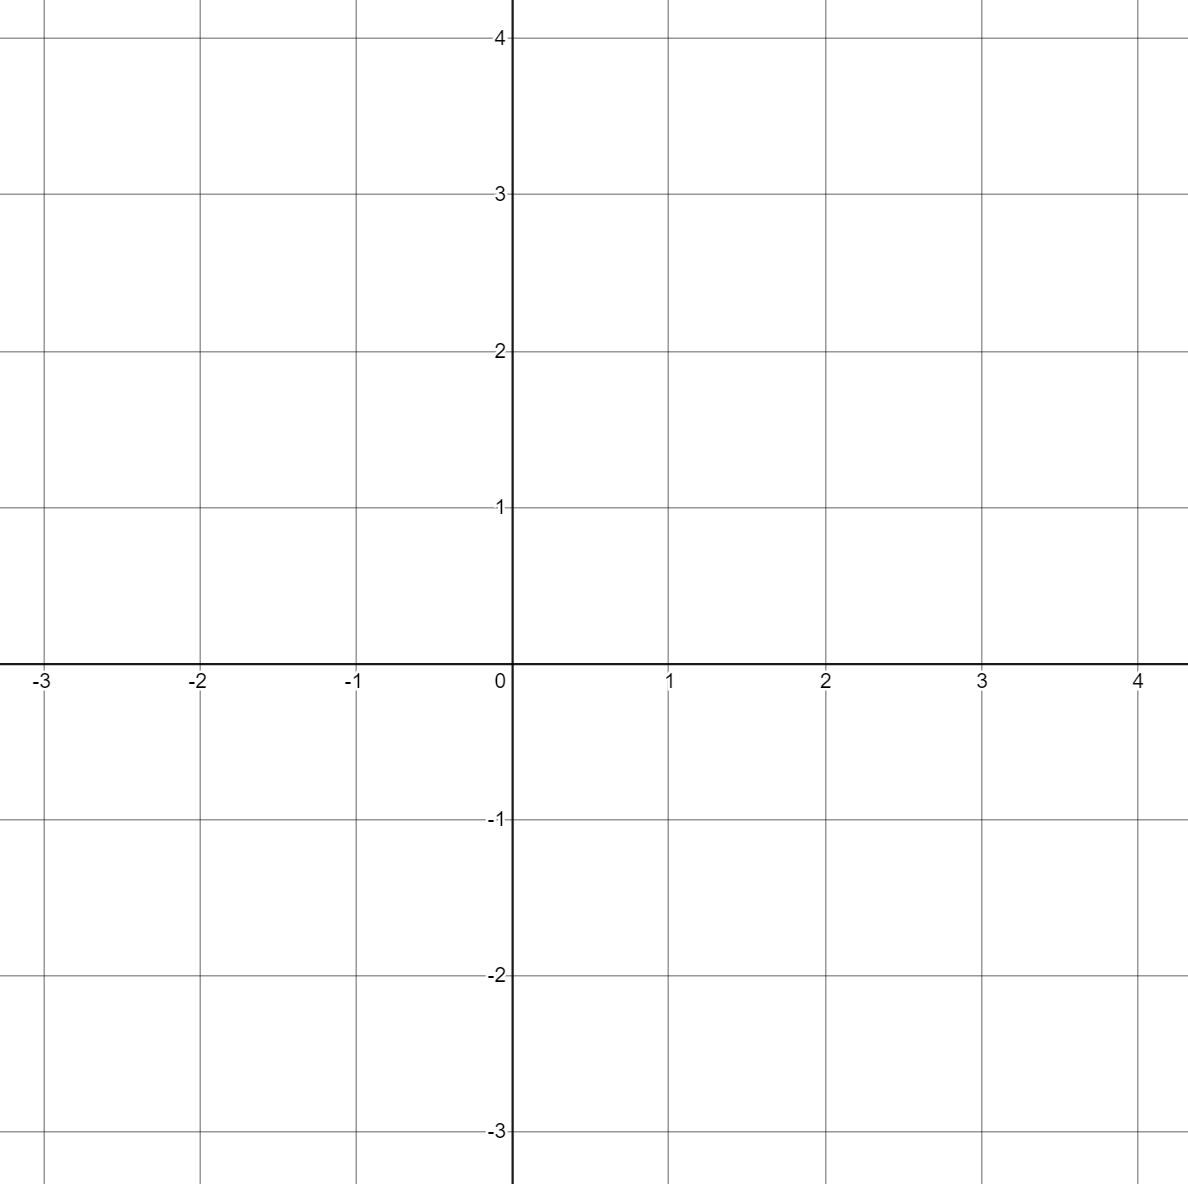
\includegraphics[width=4in]{10-09P_axes.png}
                \end{center}
        \item What do you think the formula for this graph is?
        \end{enumerate}
\end{exercise}

\newpage

\begin{exercise}
        Use the limit definition of the derivative to compute $f'(x)$ for $f(x) = x^2-x-2$.
        Do your results match your results from Exercise 1?\\
        $f'(x) = \dlim_{h \to 0}\dfrac{f(x+h) - f(x)}{h} = $
        \vfill
\end{exercise}

\begin{exercise}
        Desmos offers an interactive applet that gives a good visual and tactile experience of poroducing the derivative function point by point.
        Follow the link below and follow the instructions, using the function $f(x) = \sin x$.\\
        \url{https://www.desmos.com/calculator/jlcpl1spy2}\\
        In the space below, sketch the graphs of $f(x)$ and $f'(x)$. Do you recognize the graph of $f'(x)$?
        \vfill
\end{exercise}

\newpage

\section{Differentiability}

If the limit defining $f'(a)$ exists, we say $f$ is \textbf{differentiable} at $x=a$.

\begin{theorem}
        If $f(x)$ is differentiable at $x = a$, then it is also continuous there.
        However, the converse is \textbf{not} true: a function may be continuous at a point, but not differentiable there
        (e.g. $f(x) = |x|$ is continuous at $x = 0$, but is not differentiable there).
\end{theorem}

What might go wrong? Any of the things that make a limit not exist.
In paticular:
\begin{enumerate}[(a)]
\item the left-hand limit might not equal the right-hand limit.
\item the limit might be infinite.        
\end{enumerate}

\begin{exercise}
        Sketch the graph of a continuous function that is differentiable everywhere \textbf{except}:
        \begin{itemize}
        \item at $x = 1$ because the limit DNE as in (a) above (the derivative from the left does not equal the derivative from the right)
        \item at $x = 4$ because the limit DNE as in (b) above (the derivative is infinite)
        \end{itemize}
        \vfill
\end{exercise}


\begin{notation}
        The derivative of a function $f(x)$ has a second notation, namely
        \[
                f'(x) = \dfrac{dy}{dx}
                \qquad \qquad
                f'(a) = \left.\dfrac{dy}{dx}\right|_{x = a}
        \]
        This alterantive notation $\dfrac{dy}{dx}$ is read as ``the derivative of $y$ with respect to $x$'',
        and is called \textbf{Leibniz notation}.
        It reminds us that the derivative is the slope:
        \[
                m \equiv \dfrac{\Delta y}{\Delta x}
                \qquad
                \mbox{so}
                \qquad
                f'(x) = \dfrac{dy}{dx}
        \]
        Leibniz notation also helps to represent taking the derivatives as an operation:
        the symbol $\dfrac{d}{dx}$ means ``take the derivative with respect to $x$''.
        % For example,
        % \[
        %         \dfrac{d}{dx}(mx+b) = m
        % \]
        % since the derivative of a linear function is just the slope of the original line.
\end{notation}


\begin{exercise}
        Use the limit definition of the derivative to prove that the derivative of a line is its slope:\\
        $\dfrac{d}{dx} \left(mx+b\right) = $
        \vfill                
\end{exercise}


\end{document}
